\documentclass{beamer}
\mode<presentation> 
{
	\usetheme[alternativetitlepage]{Torino}
	\usecolortheme{chameleon}
	\setbeamercovered{transparent}	
}
\usepackage{ucs}
\usepackage[utf8x]{inputenc}
\usepackage[czech]{babel}
\usepackage{palatino}
\usepackage{graphicx}
\usepackage{epstopdf}
\usepackage{color}
\usepackage[export]{adjustbox}
\usepackage{multicol}
\usepackage{hyperref}
\usepackage{caption}
\usepackage{subcaption}




\definecolor{olive}{RGB}{51, 149, 48}
\definecolor{red}{RGB}{195, 2, 36}

\title{\textbf{Digitální fotografie}}
\subtitle{Snímače, RAW a zpracování obrazu}
\author{Pavel Macenauer \\ \tiny{pavel.macenauer@fotoaparat.cz}}
\date{\tiny{\today}}
\institute[FIT VUTBR]
{
	\inst{}
	Fakulta Informačních Technologií \\
	Vysoké Učení Technické v Brně
}

\begin{document}

	\begin{frame}[t,plain]
	\titlepage
	\tableofcontents[currentsection]
	\vspace{-7mm}
	\center{ 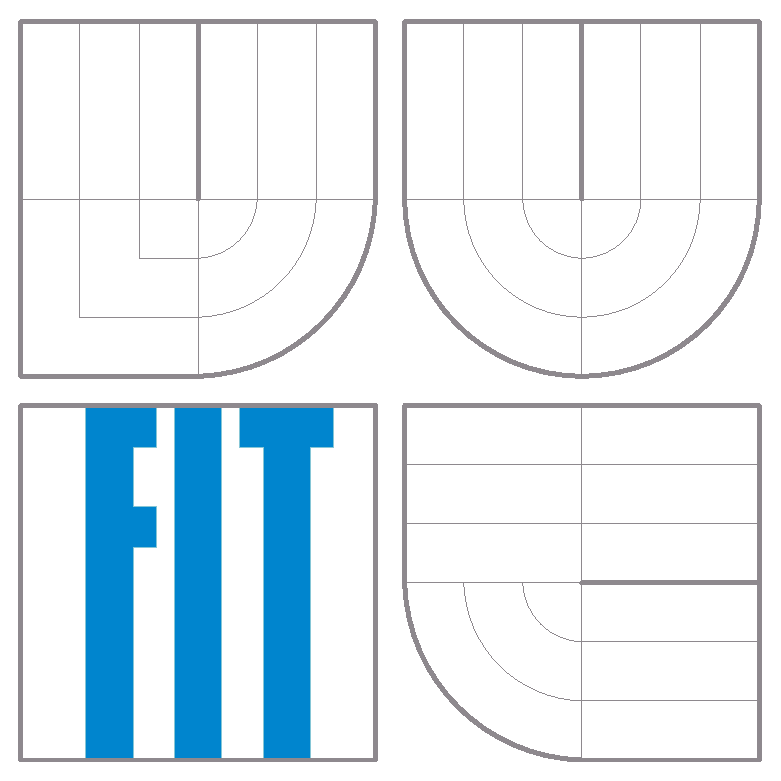
\includegraphics[height=11mm]{logo.eps} }
	\end{frame}

%% ------------- SNIMAC -------------

	\begin{frame}[t,fragile]
		\frametitle{Snímač}	
		
		\begin{itemize}
			\item destička pokrytá snímacími body (př. 10 Mpix - 10 mil. bodů), rozměry se liší pro jednotlivé modely, nejčastěji 3x2
			\item \textcolor{red}{CMOS} nebo \textcolor{red}{CCD}	
			\item před snímacími body je \textcolor{red}{barevná maska} (CFA) pro výpočet barvy
			\item \textit{\textcolor{red}{režim live view} (u zrcadlovek): odklopí se zrcátko a senzor generuje náhled}
			\begin{itemize}
				\item softwarový autofokus
			\end{itemize}
		\end{itemize}	
		

		\vspace{-8mm}\center\begin{tabular}{ll}
			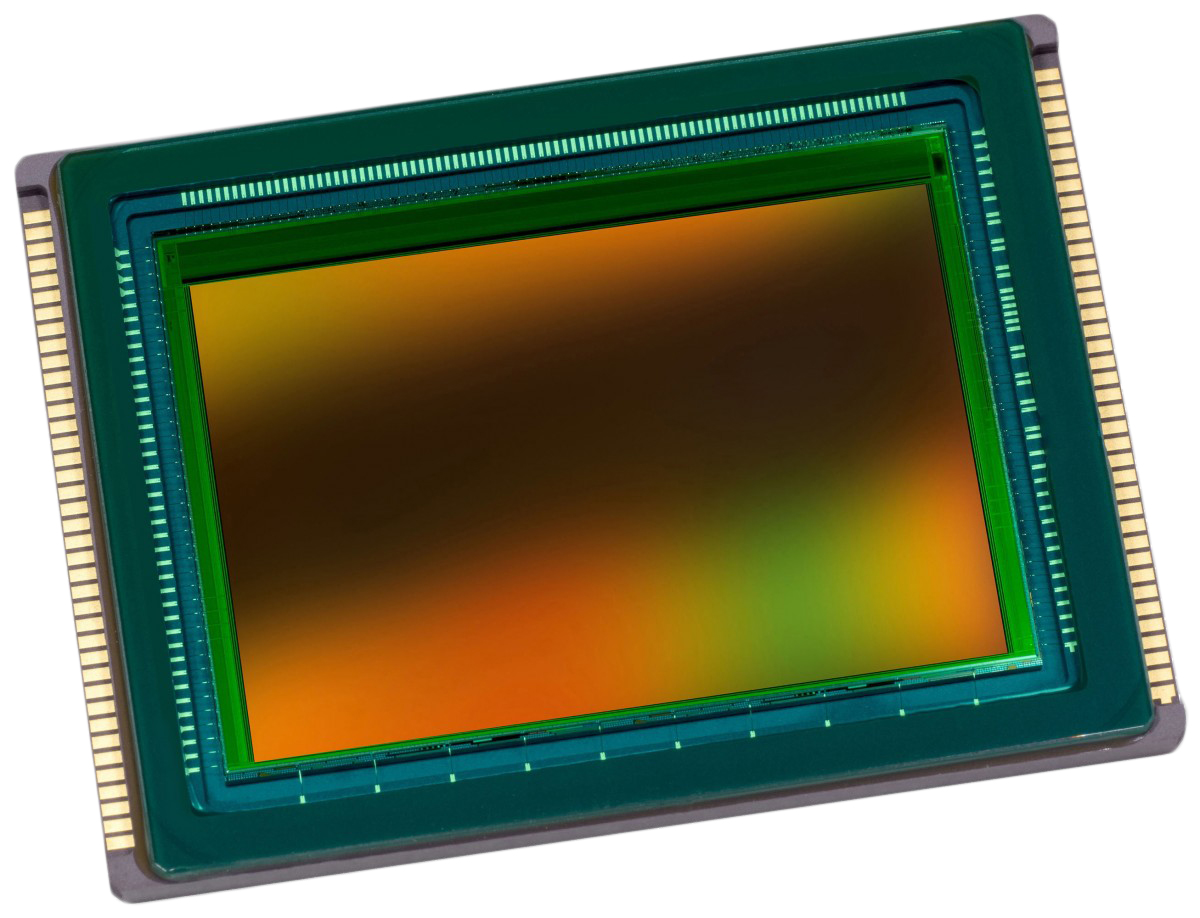
\includegraphics[height=30mm]{cmos-real.jpg} &		
			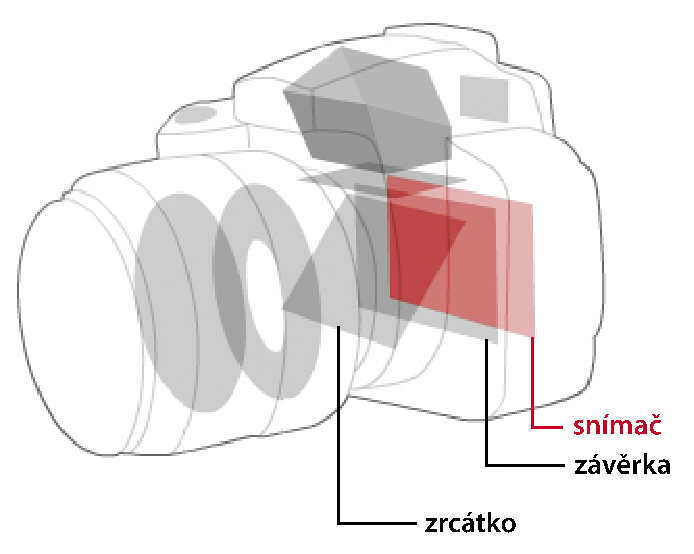
\includegraphics[height=40mm]{sensor.pdf}

		\end{tabular}

				
	\end{frame}
	
%% -------------- CCD ----------------

	\begin{frame}[t,fragile]
		\frametitle{CCD - Charged Couple Device}
		\begin{tabular}{ll}
			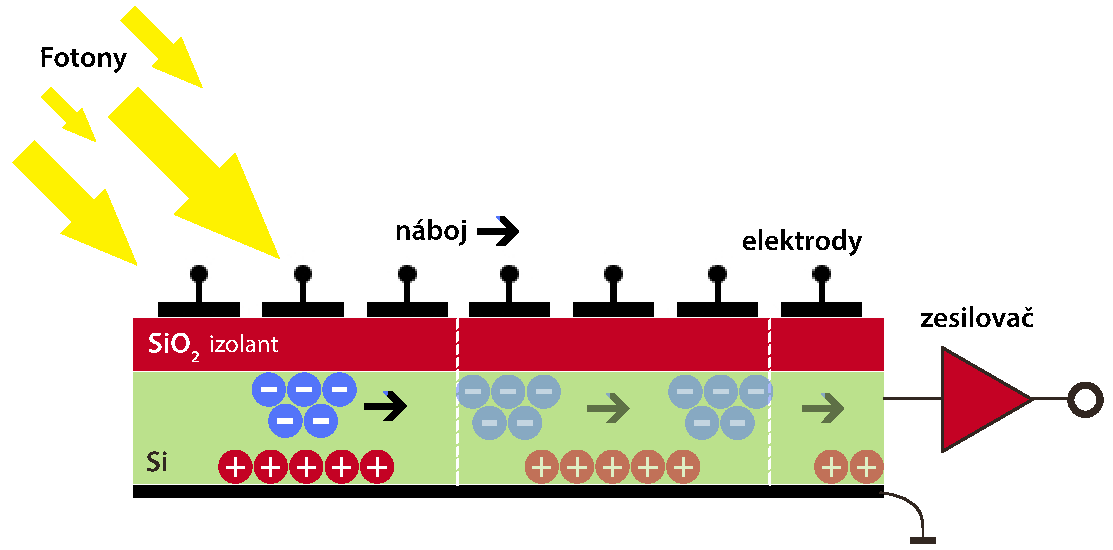
\includegraphics[height=35mm]{ccd.pdf} &		
			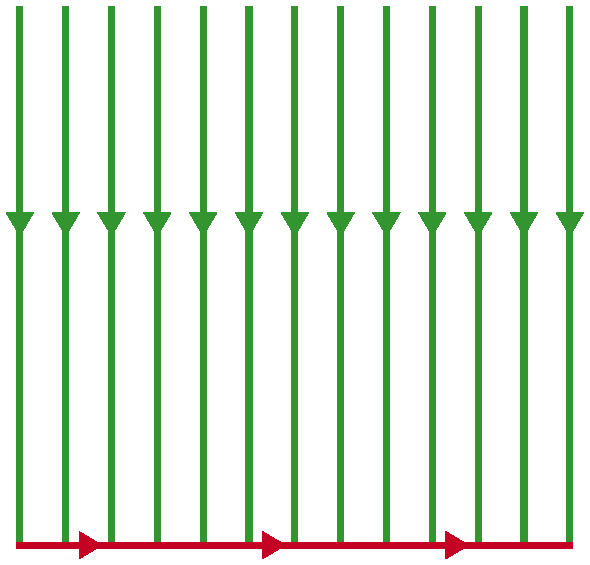
\includegraphics[height=30mm]{2dccd.pdf}
		\end{tabular}
		\begin{enumerate}		
			\item otevře se závěrka a na \textcolor{red}{polovodič} dopadají fotony generující elektrony/díry
			\item závěrka se uzavře a postupně se nabíjejí elektrody, které posouvají náboj směrem k zesilovač
			\item zesilovač zesílí proud na zpracovatelnou napěťovou úroveň
		\end{enumerate}	
		
	\end{frame}
	
%% -------------- CMOS ----------------

	\begin{frame}[t,fragile]
		\frametitle{CMOS - Complementary Metal-Oxide Semiconductor}	


		\centering\begin{tabular}{ll}
			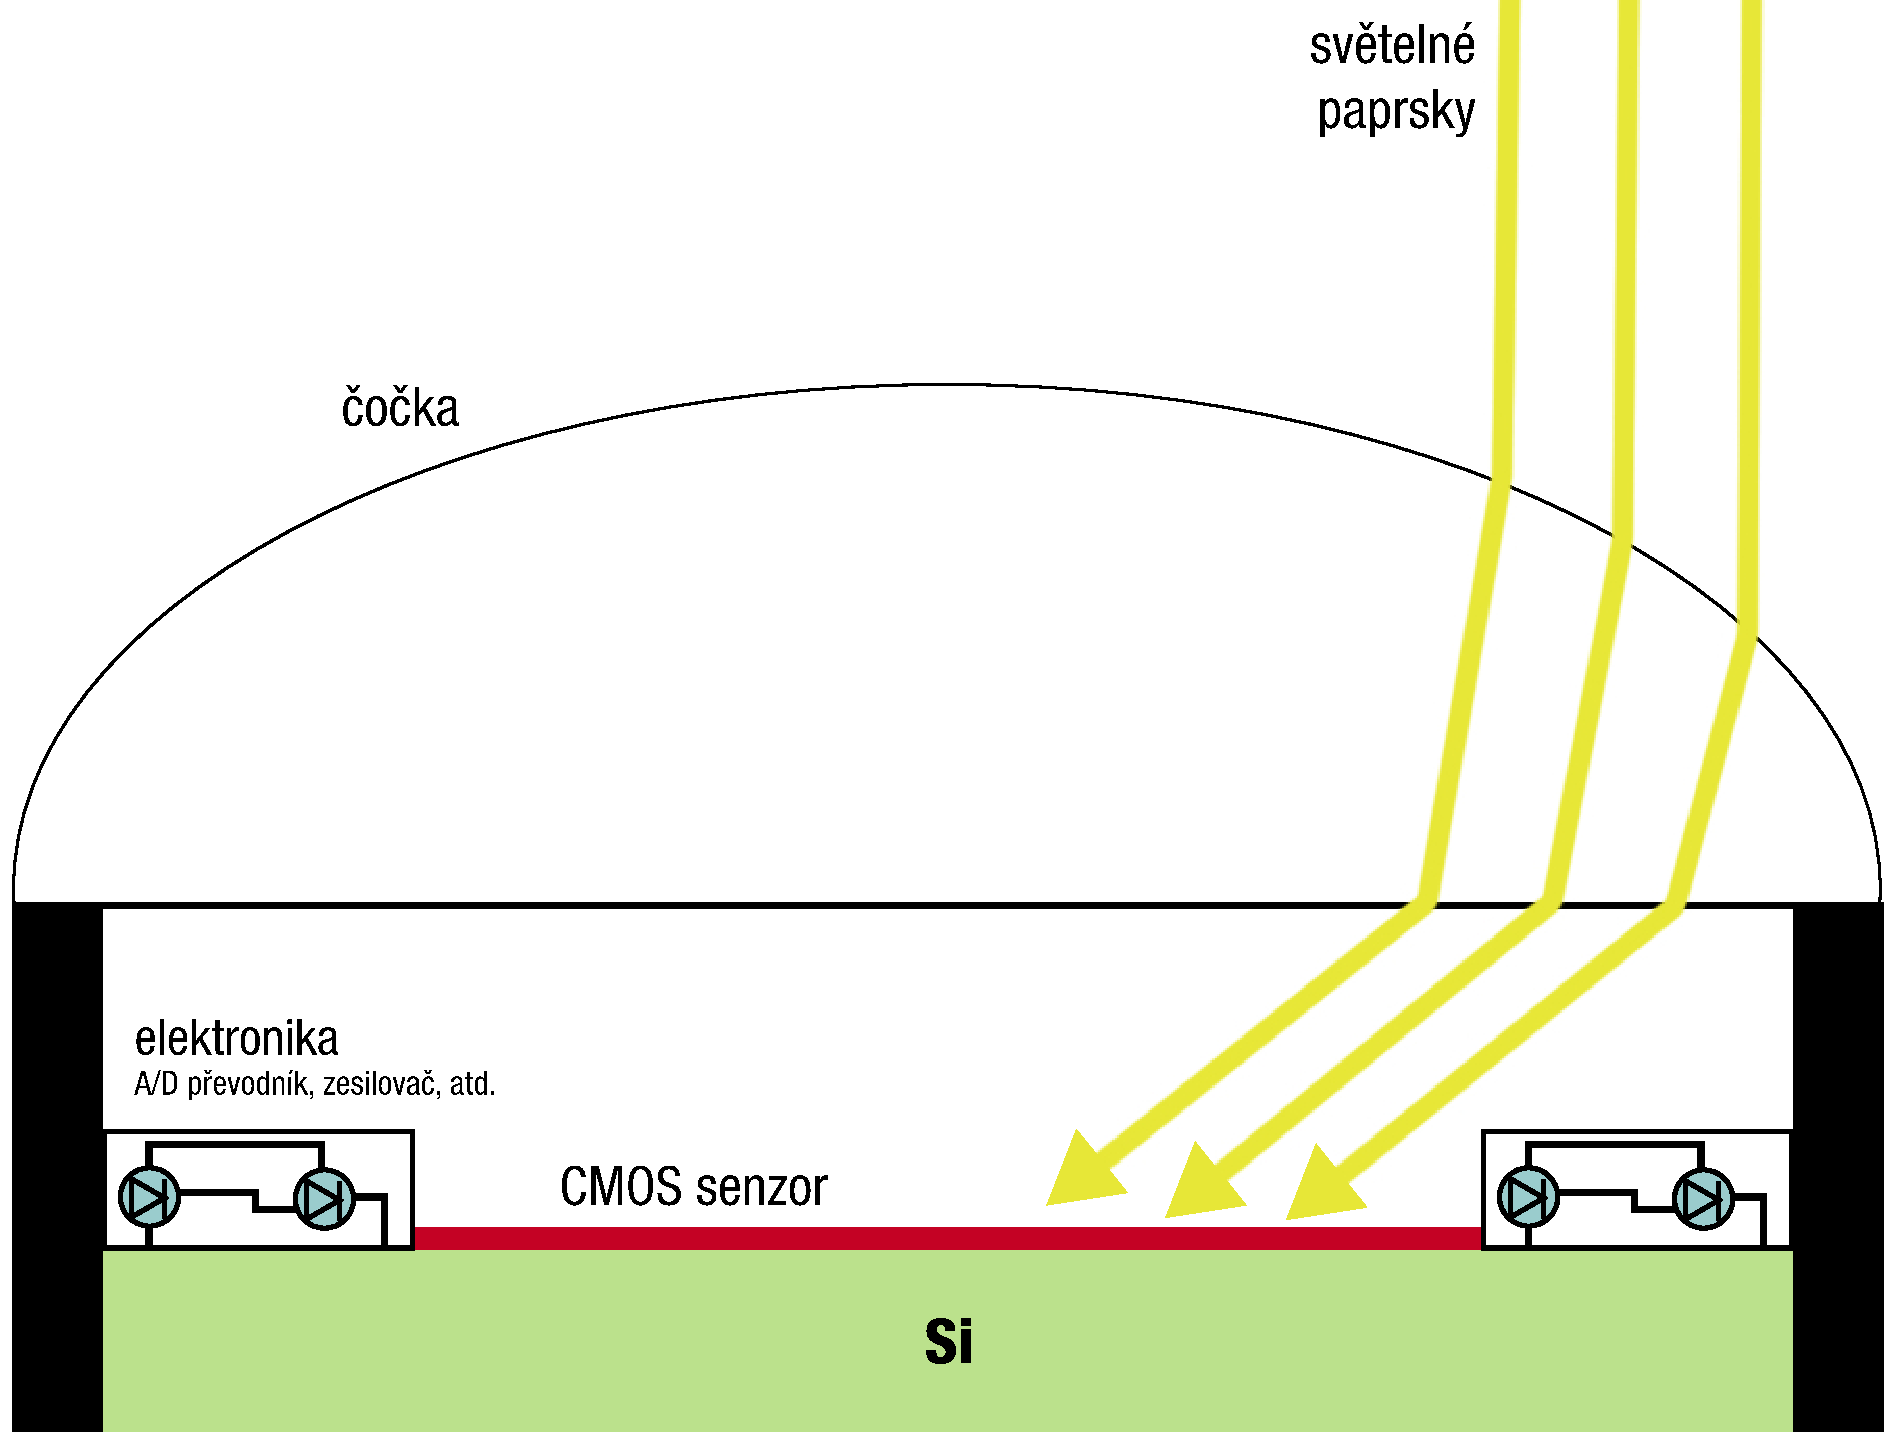
\includegraphics[width=55mm]{cmos-schema.pdf} &		
			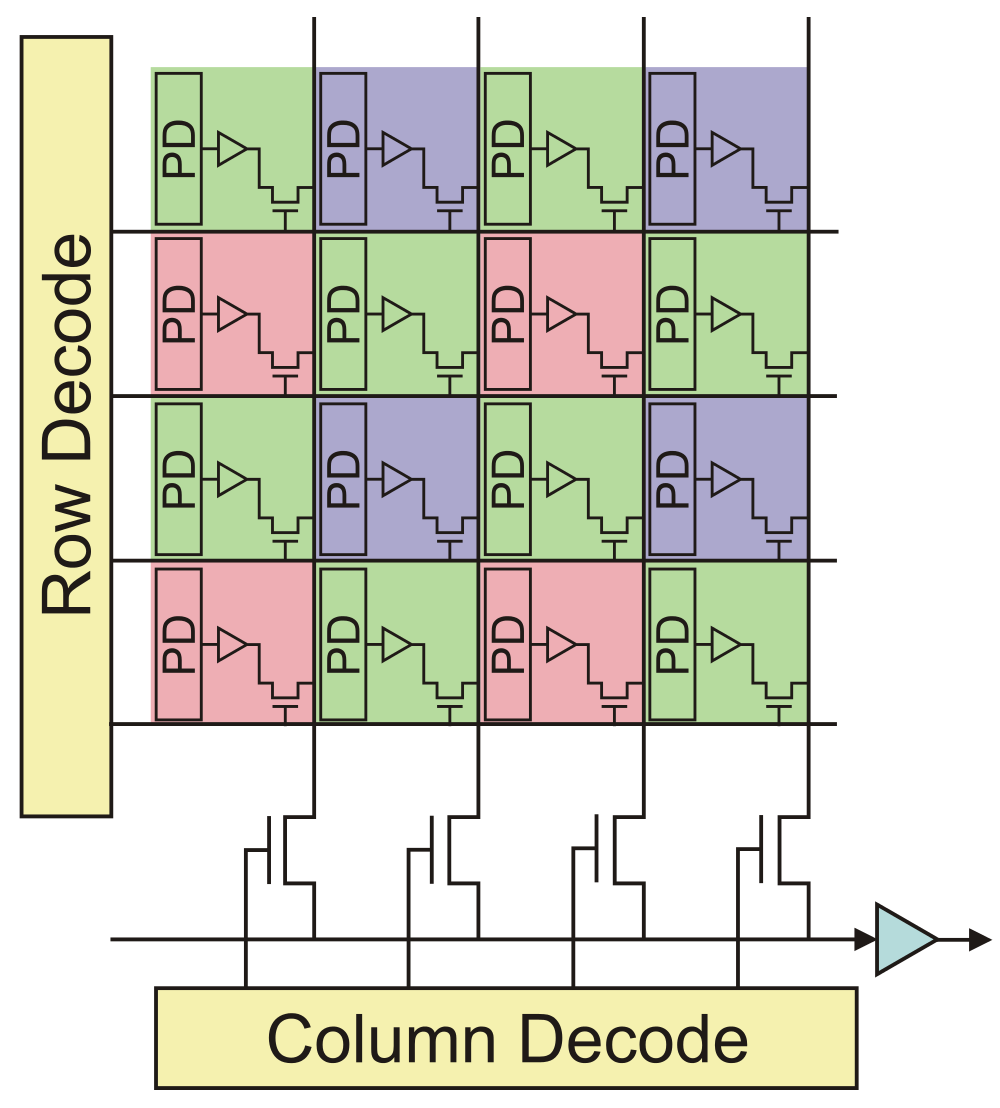
\includegraphics[width=35mm]{cmos-address.png}
		\end{tabular}
		
 
		\begin{itemize}		
			\item na každé buňce \textcolor{red}{fotodioda}, A/D převodník a zesilovač
			\item přímá adresace jednotlivých buněk umožňující více virtuálních obrazovek, rychlejší čtení (fps) a následné zpracování, ...
			\newline
			
		\end{itemize}			

	\end{frame}
	
%% -------------- CMOS vs CCD ----------------

	\begin{frame}[t,fragile]
		\frametitle{CMOS vs. CCD}					
		\begin{itemize}
	    	\item \textcolor{olive}{Výhody CMOS}				
	    	\begin{itemize}
				\item \textcolor{red}{levnější na výrobu}, \textcolor{red}{menší spotřeba} (až 100x) - nižší teploty
				\item rychlejší zpracování - \textcolor{red}{přímý diskrétní výstup} umožňuje rychlejší zpracování a především natáčení videa
				\item odolnost proti \textcolor{red}{bloomingu} - přetékání světla do okolních pixelů
	    	\end{itemize}

			\item \textcolor{olive}{Výhody CCD}
			\begin{itemize}
				\item \textcolor{red}{lepší obrazová kvalita} (CCD může mít více bodů na stejnou plochu), nemá elektroniku na chipu, která by snižovala množství dopadajícího světla + je citlivější
				\item lepší funkčnost za \textcolor{red}{špatných světelných podmínek} a méně šumu
				
			\end{itemize}
		\end{itemize}	
		
		\textcolor{red}{CMOS} senzory se rychle vyvíjejí, viz. např. \textcolor{red}{BIS CMOS} a mají je dnes téměř všechny \textcolor{red}{DSLR}.
	\end{frame}
	
% ------------------ CFA -----------------
	
	\begin{frame}[t,fragile]
		\frametitle{Color Filter Array (CFA)}	
		
		\begin{itemize}
			\item proč? senzory \textcolor{red}{neměří vlnovou délku} světla - barvu
			\item přes senzor je umístěna mozaiková struktura různých barevných filtrů (čtveřice barev)
			\item \textcolor{red}{Bayer} (RGGB, na zelenou je lidské oko nejcitlivější), RGBE, CYYM, CYGM, RGBW, ...
			\item \textit{Foveon - všechny 3 vrstvy na sobě umožňující úplnou barevnou informaci, používá Sigma}

		\end{itemize}			
		
		\vspace{-3mm}\center\begin{tabular}{lll}
			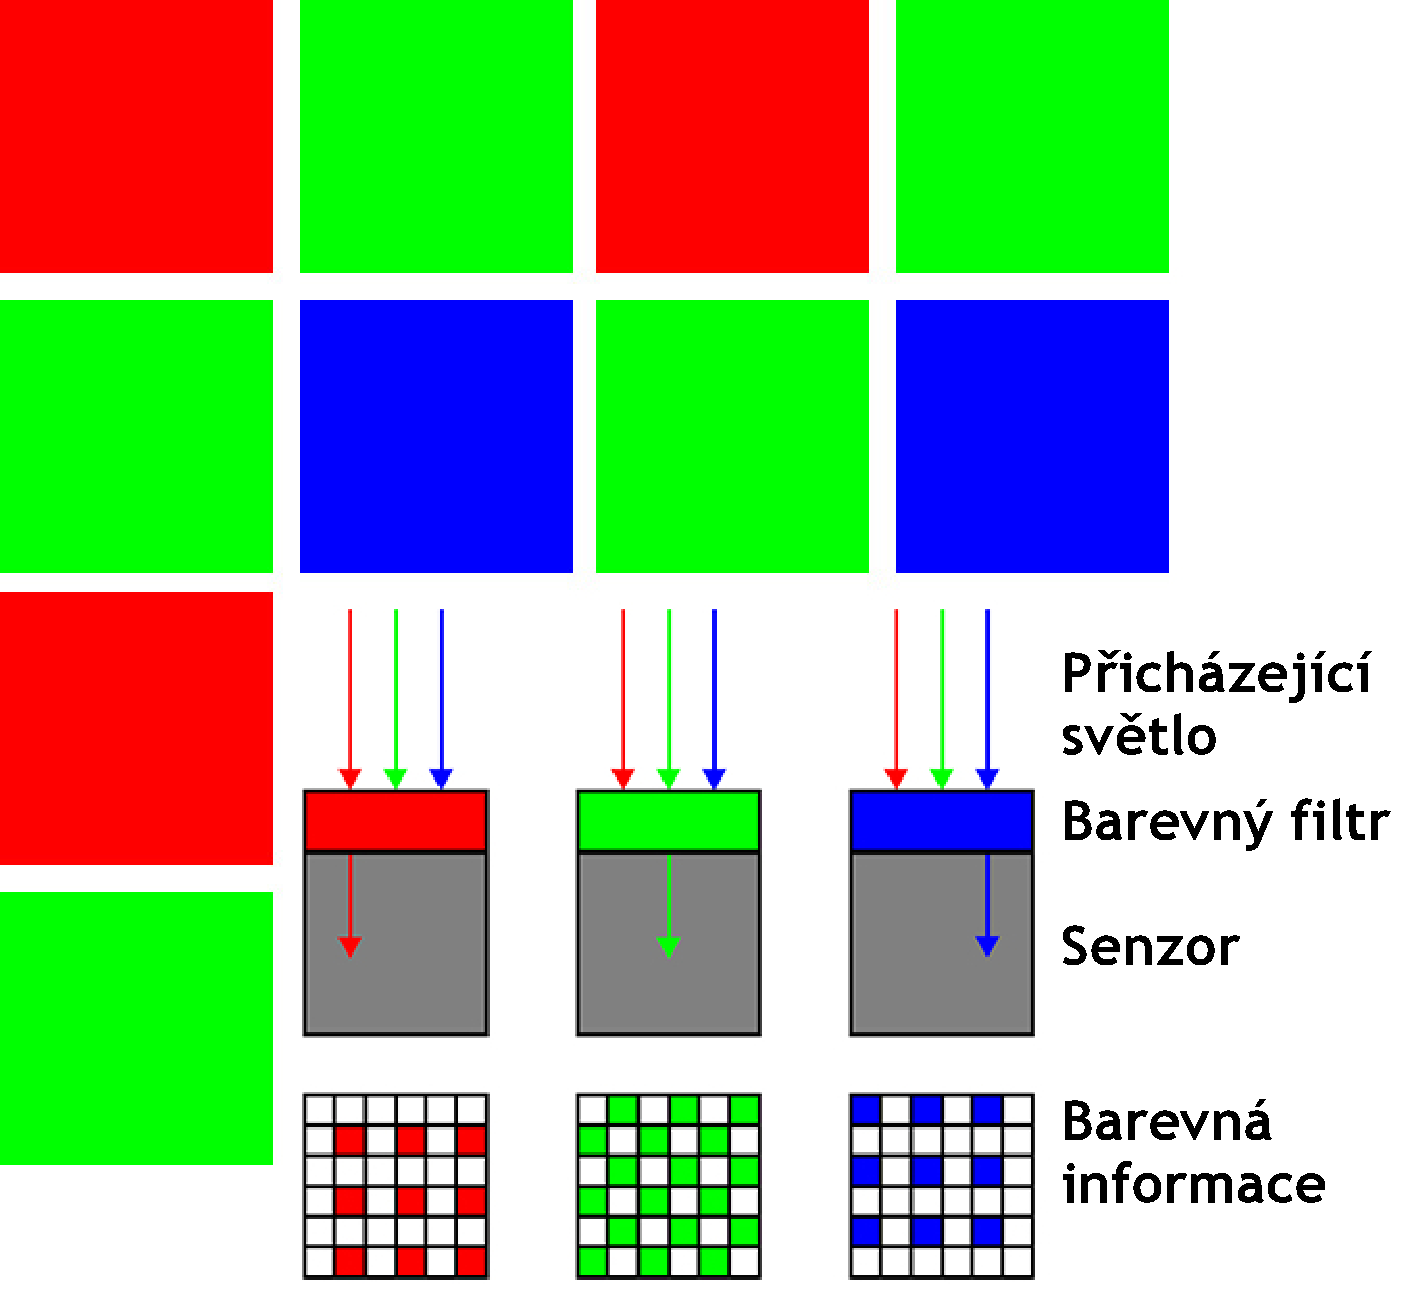
\includegraphics[height=30mm]{bayer-mask.pdf} &		
			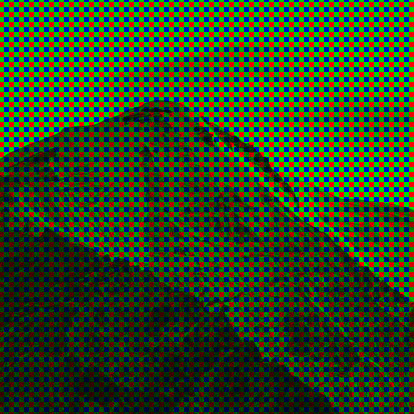
\includegraphics[height=30mm]{bayer-image.jpg} &
			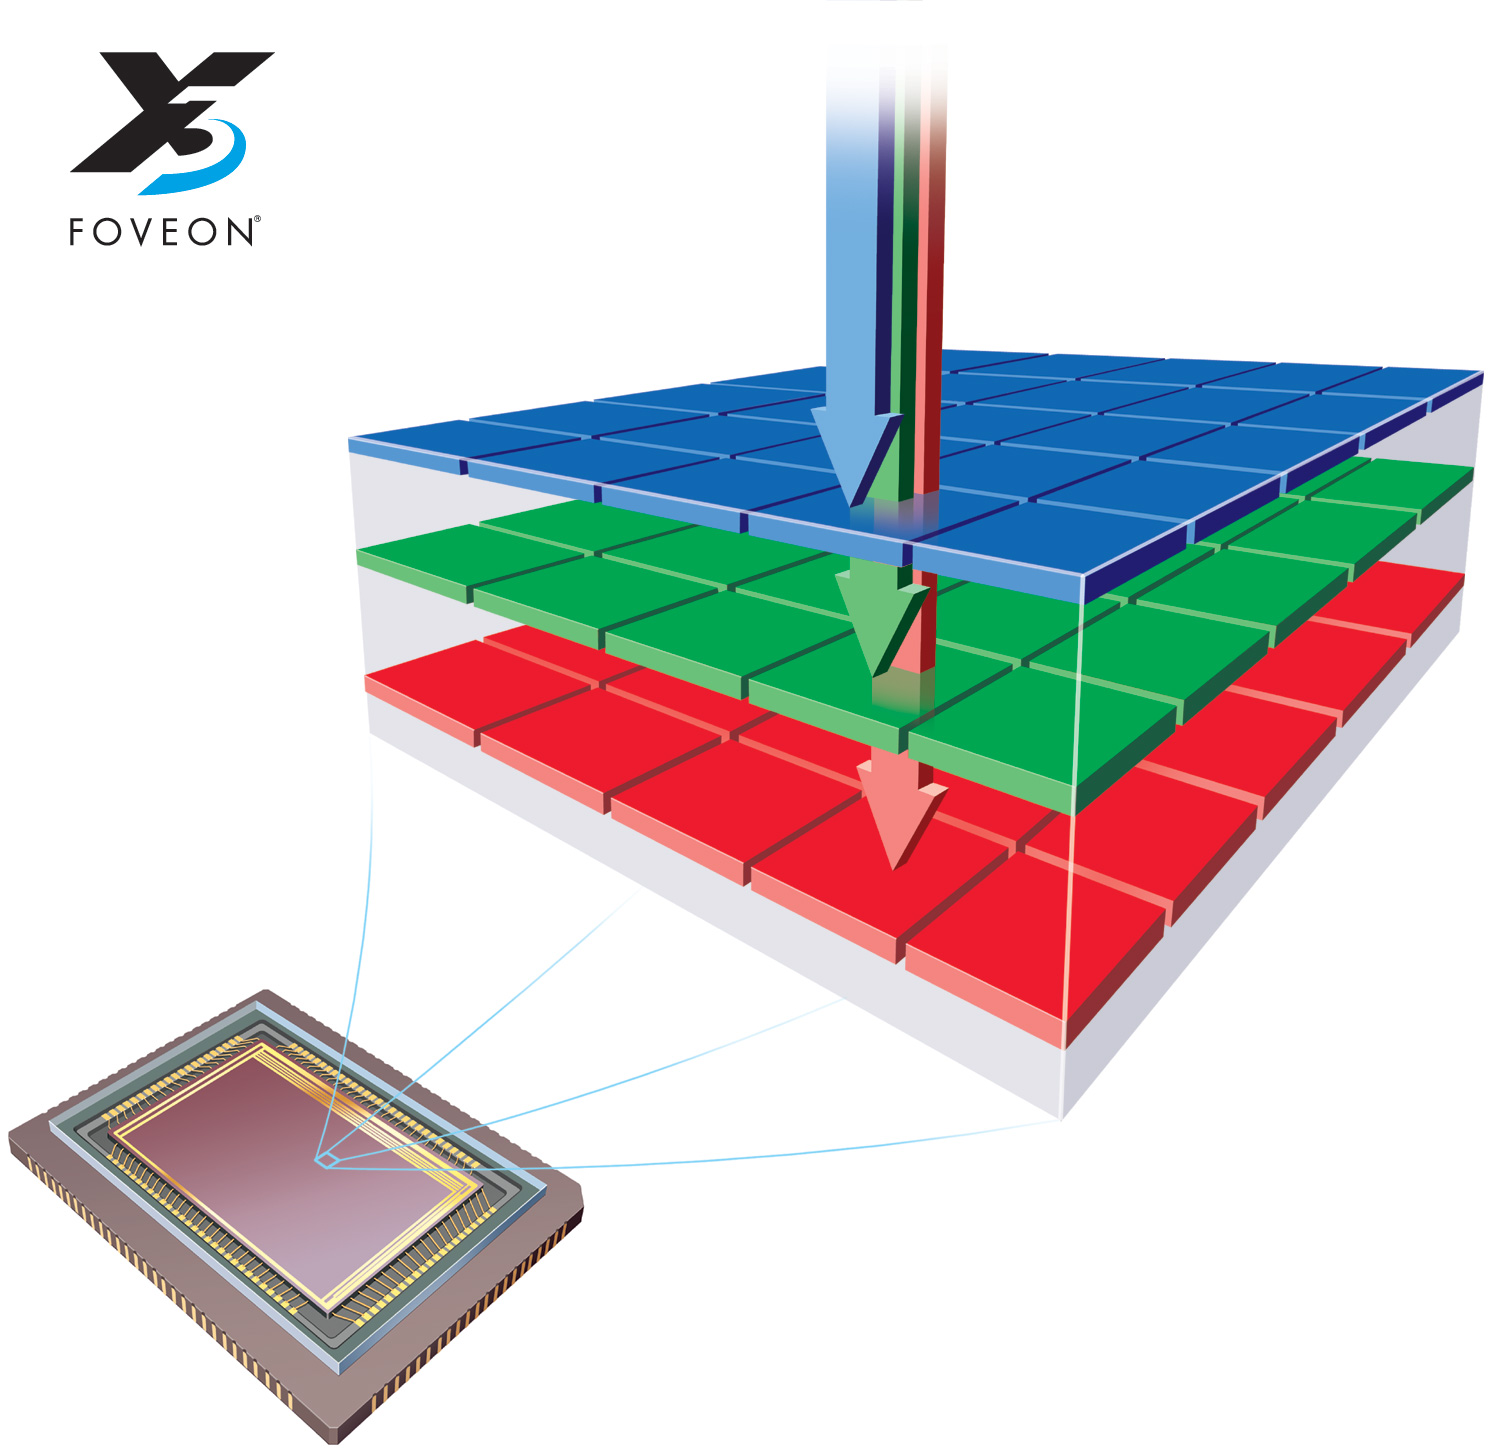
\includegraphics[height=30mm]{foveon-cfa.jpg}
		\end{tabular}		
				
	\end{frame}	
	
	
	%% -------------- RAW ----------------
	
		\begin{frame}[t,fragile]
		\frametitle{Co je to Raw \textit{[ró]}?}
		
		\begin{itemize}
			\item nejedná se o zkratku, ale že se jedná o \textcolor{red}{surový výstup}
			\item není to obraz, ale \textcolor{red}{data sloužící k vytvoření obrazu} (digitální temná komora, \verb!dng! = Digital Negative)
		
			\item formáty: \verb!dng! (Adobe, Pentax), \verb!cr2! (Canon), \verb!nef! (Nikon), \verb!orf! (Olympus), ...
			\item pokus Adobe o to standardizovat \verb!dng! se nepovedl
			\item obsahuje obrazová data a metadata (TIFF-EP, EXIF, IPTC, XMP + proprietární metadata), profil fotoaparátu, opcode lists

		\end{itemize}	
			
		\vspace{-6mm}\center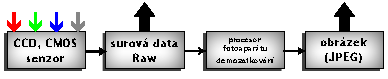
\includegraphics[width=110mm]{chain.pdf}
		\vspace{3mm}
				
	\end{frame}		
	
	%% -------------- DEMOZAIKOVANI ----------------	
	
	\begin{frame}[t,fragile]
		\frametitle{Demozaikování}		
		\textcolor{red}{Vytvoření bitmapy/obrazu} ze surových dat.

			\begin{itemize}
				\item \textcolor{red}{vytvoření barvy} - interpolace ze sousedních pixelů
				\item doostření, \textcolor{red}{vyvážení bílé} (barevná teplota), jasu, kontrastu

			\end{itemize}

		
		\center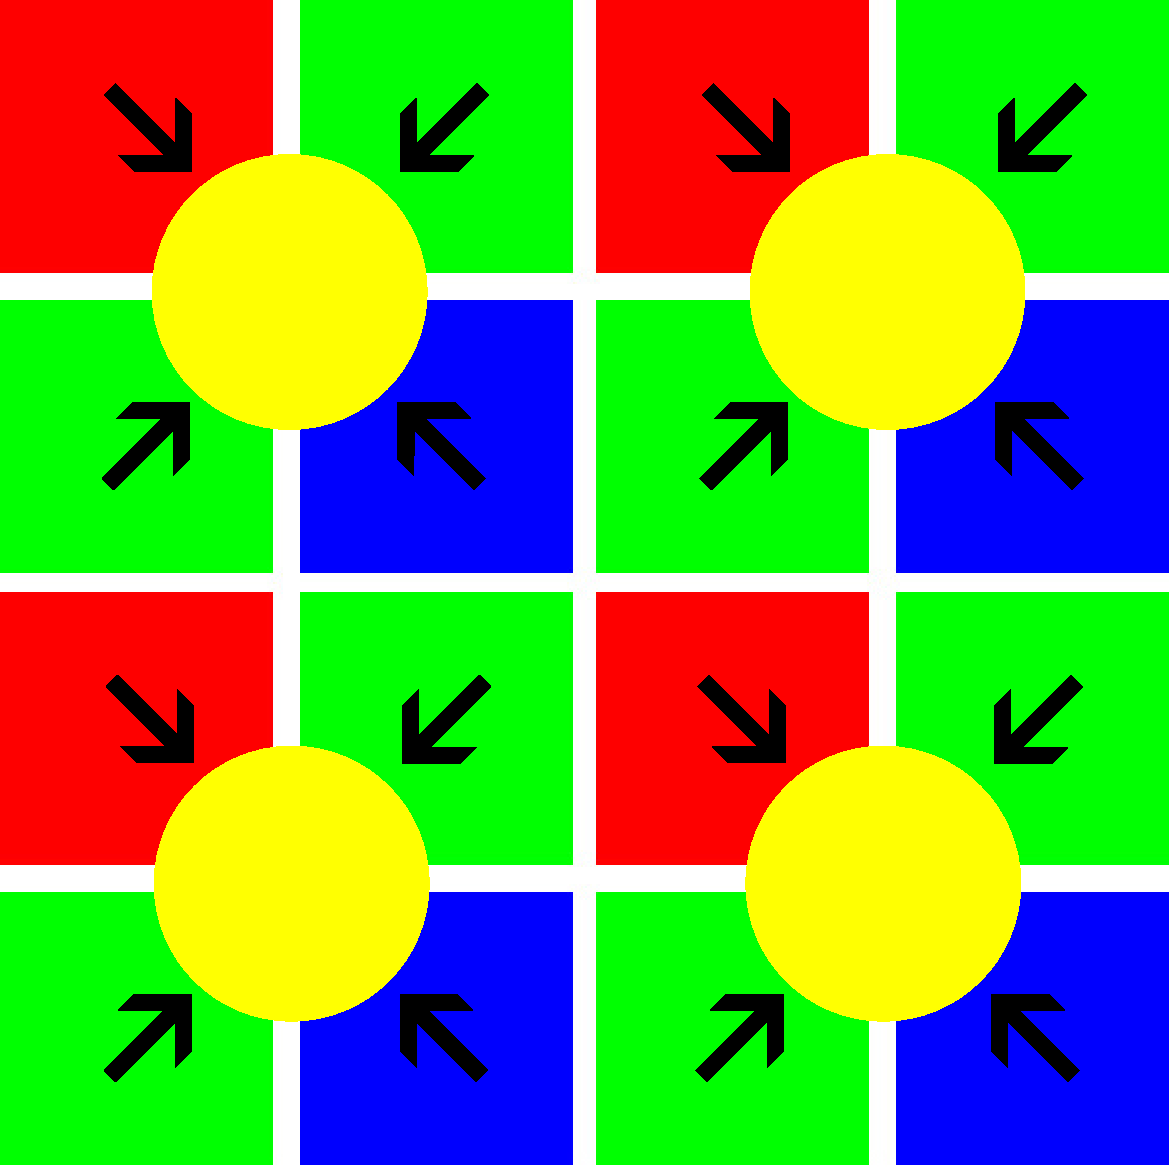
\includegraphics[height=25mm]{bayer-interpolation.pdf}		
		\begin{itemize}	
			\item mapování na 8/16-bit barevnou hloubku a přiřazení ICC profilu
			\item redukce vad objektivu (chromatická aberace, vinětace, soudkovitost, atd.)
		\end{itemize}
		
	\end{frame}	
	
	% ------------------ Demozaikovani -----------------
	
	\begin{frame}[t,fragile]
		\frametitle{Demozaikování - příklad}	
		
				
		\begin{figure}[htbp]
        \centering

        \begin{subfigure}[b]{0.32\textwidth}
                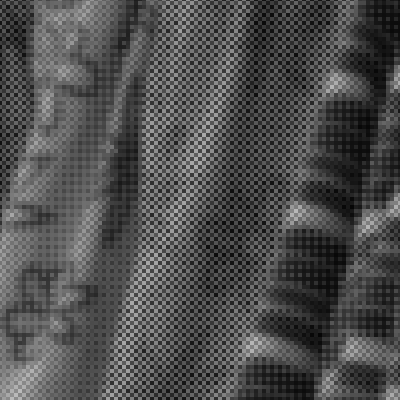
\includegraphics[width=\textwidth]{e_nonwb.png}
                \caption{\scriptsize{Před vyvážením bílé}}
        \end{subfigure}   
        \begin{subfigure}[b]{0.32\textwidth}
                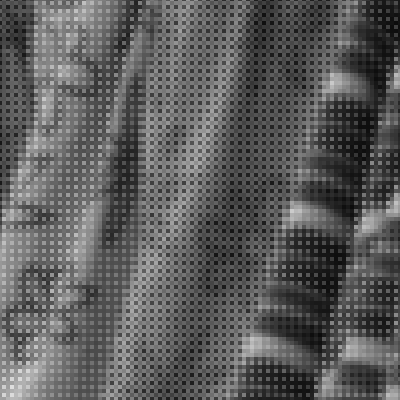
\includegraphics[width=\textwidth]{e_wb.png}
                \caption{\scriptsize{Po vyvážení bílé}}

        \end{subfigure}
        \begin{subfigure}[b]{0.32\textwidth}
                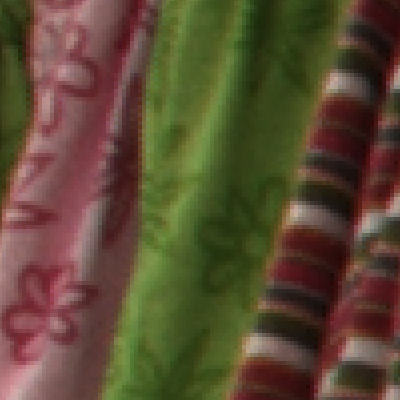
\includegraphics[width=\textwidth]{e_demosaiced.png}
                \caption{\scriptsize{Demozaikováno}}

        \end{subfigure}
        \end{figure}
    

				
				
	\end{frame}	
	
	%% -------------- vyhody nevyhody ----------------			
	
	\begin{frame}
		\frametitle{Výhody a nevýhody}

			\begin{itemize}
	    	\item \textcolor{olive}{Výhody}
	    		\begin{itemize}
	    			\item \textcolor{red}{zpracování v 12/14-bit barevné hloubce} (podle výrobce senzoru) - umožňuje širší dynamický rozsah, než-li 8-bit JPEG
	    			\item vlastní nastavení doostření, barevné teploty, jasu, kontrastu
	    			\item \textcolor{red}{nedestruktivní úprava} - informace o úpravách se ukládají buď do externího XMP souboru nebo přímo do RAW
	    		\end{itemize}	
	    	\end{itemize}    	

	    	\begin{itemize}
    		\item \textcolor{red}{Nevýhody}
	    		\begin{itemize}
	    			\item velké soubory (vyjímka 16-bit TIFF, který je větší)
	    			\item časová náročnost zpracování
	    			\item kompatibilita RAW konvertorů a novějších fotoaparátů (DNG Convertor)
	    		\end{itemize}
			\end{itemize}

	\end{frame}
	
	%% -------------- raw konvertory ----------------				
	
	\begin{frame}
		\frametitle{Raw konvertory}
		\begin{itemize}
	    	\item Adobe Camera Raw (Adobe Lightroom, plug-in do Adobe Photoshop), Zoner Photo Studio
	    	\item Software výrobce fotoaparátu
	    	\item Firmware fotoaparátu  			
	    \end{itemize}    	
	\end{frame}	
		
	
	% ------------------ literatura -----------------	
	
	\begin{frame}
		\frametitle{Literatura}
		\begin{enumerate}
			\scriptsize
	    	\item \textbf{Digital Negative (DNG) Specification, Adobe, June 2009} \newline \url{http://www.adobe.com/content/dam/Adobe/en/products/photoshop/pdfs/dng_spec.pdf}	    	
	    	\item \textbf{R. Sumner: Reading RAW files into MATLAB and Displaying Them, University of California, Feb. 2014\newline}\url{http://users.soe.ucsc.edu/~rcsumner/rawguide/}

			\item CCD and CMOS sensor technology - Technical White Paper, Axis Communications, 2010\newline\tiny{\url{http://www.axis.com/files/whitepaper/wp_ccd_cmos_40722_en_1010_lo.pdf}}\scriptsize
			\item R. Jean: Demosaicing with The Bayer Pattern, University of North Carolin, Nov. 2011\newline\url{http://www.unc.edu/~rjean/demosaicing/demosaicing.pdf}
	    	\item V. Zyka: RAW formát v digitální fotografii, FEL ČVUT, 2009\newline\url{http://cmp.felk.cvut.cz/cmp/courses/Y33DIF/2009-2010LS/labs/10_raw/raw.pdf}
	    \end{enumerate}    	
	\end{frame}
	
\end{document} 
